\section{Theorie}
	
Im Folgenden sollen zunächst die theoretischen Grundlagen für die nachfolgenden experimentellen Untersuchungen erörtert werden.
Die vorgestellte Theorie basiert auf der ausgehändigten Versuchsanleitung \cite{wwu}.

\subsection{Fermigasmodell des Atomkerns}
Eine Möglichkeit, einen Atomkern modellhaft zu beschreiben, bildet das Fermigasmodell, benannt nach Enrico Fermi.
Der Kern wird dabei als freies Nukleonengas beschrieben.
Die Nukleonen wechselwirken untereinander nicht, sondern befinden sich in zwei Potentialtöpfen, einer für die Protonen und einer für die Neutronen.
Im Gegensatz zum Vielelektronenproblem in der Atomphysik, handelt es sich bei Neutronen und Protonen um unterscheidbare Teilchenarten, weshalb sie in zwei unterschiedlichen Potentialtöpfen sitzen.
In den Potentialtöpfen werden die möglichen Zustände bis zur Fermi-Energie $E_F$ aufgefüllt.
Für symmetrische Kerne ist diese:
\begin{align*}
E_F\approx \SI{33}{\mega\electronvolt}.
\end{align*}
Da es sich bei Protonen und Neutronen um Fermionen handelt, können die verschiedenen Energieniveaus nur von jeweils zwei Teilchen mit gegensätzlichem Spin besetzt werden.
Außerdem ist der Potentialtopf der Protonen nicht so tief wie der der Neutronen, da die Protonen zusätzlich noch der Coulombabstoßung unterliegen.
In Abbildung \ref{fermigas} ist das Potentialschema des Fermigasmodels nocheinmal graphisch dargestellt.

\begin{figure}[h]
	\centering
	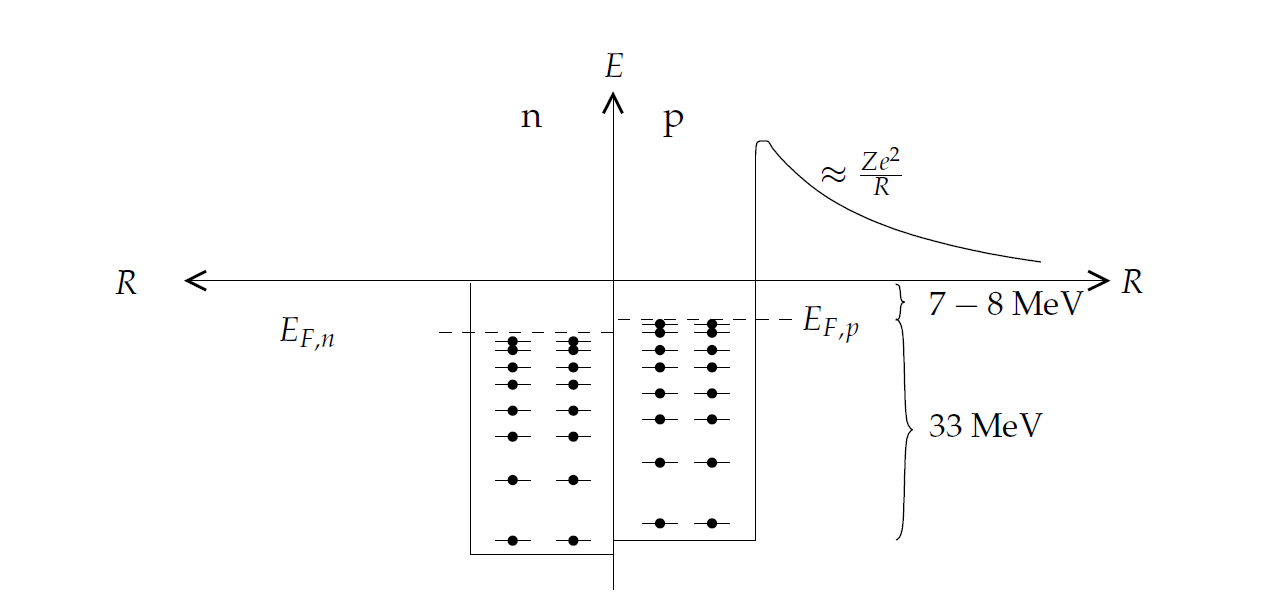
\includegraphics[width=1.0\textwidth]{img/fermigas}
	\caption{Graphische Darstellung der beiden Potentialtöpfe für Neutronen und Protonen im Fermigasmodell. \cite{fermi}}
	\label{fermigas}
\end{figure}

\subsection{Alpha-Zerfall}

Der Alpha$(\alpha) $-Zerfall wurde erstmals von Ernest Rutherford beobachtet und stellt die Emission eines Heliumkerns dar.
Er tritt nur bei relativ schweren Kernen auf.
Dies kann man durch die hohe Bindungsenergie von ca. \SI{7}{\mega\electronvolt} des Heliumkerns begründen.
Mit steigender Massenzahl $A$ nimmt die Bindungsenergie pro Nukleon ab, weshalb sich für schwere Kerne im Inneren zwei Protonen und zwei Neutronen als ein Heliumkern "abkapseln" können.
Dieser Heliumkern ist jedoch nicht frei, sondern im Kernpotential gebunden. 

Stellt man sich das Potential wie in Abbildung \ref{fermigas} nach dem Fermigasmodell vor, so befindet sich das $\alpha$-Teilchen noch im Rechteckpotential des Kerns, jedoch oberhalb der \SI{0}{\mega\electronvolt}-Linie.
Daher ist quantenmechanisch die Wahrscheinlichkeit, mit der das $\alpha$-Teilchen auf die rechte Seite des Coulombpotentials durchtunnelt ungleich null.
Diese Wahrscheinlichkeit bestimmt die Zerfallsdauer und lässt durch den sogenannten Gamow-Faktor näherungsweise berechnen.
Das Grundprinzip des Alpha-Zerfalls wird also mit dem Fermigasmodell verständlich.
Als allgemeine Zerfallsgleichung lässt er sich schreiben als:
\begin{align*}
^A_ZX_N\longrightarrow \,^{A-4}_{Z-2}Y_{N-2} \,+ \,^4_2\textnormal{He}_2
\end{align*}
Es handelt sich also um einen Zweikörperzerfall. Aus Energie- und Impulserhaltung folgt, dass die Energie der Alpha-Teilchen diskret sein muss. Es kann jedoch mehrere diskrete Energielinien geben, je nachdem ob der Tochterkern nach dem Zerfall in einem angeregten Zustand vorliegt oder nicht. 

Der Gamow-Faktor für ein Teilchen der Masse $m$ und Energie $E$ beim Tunneln durch ein Potential $V(x)$ zwischen den Punkten $a$ und $b$ ist gegeben durch:
\begin{align}
	T=\exp\left[ -\frac{2}{\hbar}\int_{a}^{b}\sqrt{2m\left( V(x)-E\right) }\,\text{d}x\right] 
\end{align}

\subsection{Wechselwirkung von Alpha-Strahlung mit Materie}

Schwere geladene Teilchen (d.\,h. keine Elektronen/Positronen) verlieren beim Durchqueren eines Festkörpers die meiste Energie durch inelastische Kollisionen mit den Elektronen des Festkörpers.
Bei sehr schweren Kernbruchstücken ist zudem die Wechselwirkung mit den Kernen des Mediums nicht zu vernachlässigen.
Die Kollisionen mit den Elektronen können zudem in weiche und harte unterteilt werden.
Bei weichen Kollisionen kommt es nur zur einer Anregung, bei harten gar zu einer Ionisation.

\subsubsection{Bethe-Bloch-Formel}

Der Energieverlust schwerer geladener Teilchen kann durch die Bethe-Bloch-Formel beschrieben werden.
Sie lautet:
\begin{align}
	\label{eq:bethebloch}
	-\dv{E}{x}=K\rho \frac{Z}{A}\frac{z^2}{\beta^2}\left[ \ln(\frac{2m_e\gamma^2v^2W_\text{max}}{I^2})-2\beta^2-\delta -2\frac{C}{Z}\right] 
\end{align}
Dabei ist $K=2\pi N_A r_e^2m_ec^2= \SI[per-mode=reciprocal-positive-first]{0.1535}{\mega\electronvolt\centi\meter\squared\per\gram}$.
Eine Erklärung aller auftauchenden Größen findet sich in der nachfolgenden Tabelle \ref{tab:bethebloch}.
Außerdem zeigt Abbildung \ref{bethebloch} einen beispielhaften Kurvenverlauf der Bethe-Bloch-Formel für Myonen in Kupfer.

\begin{figure}[h]
	\centering
	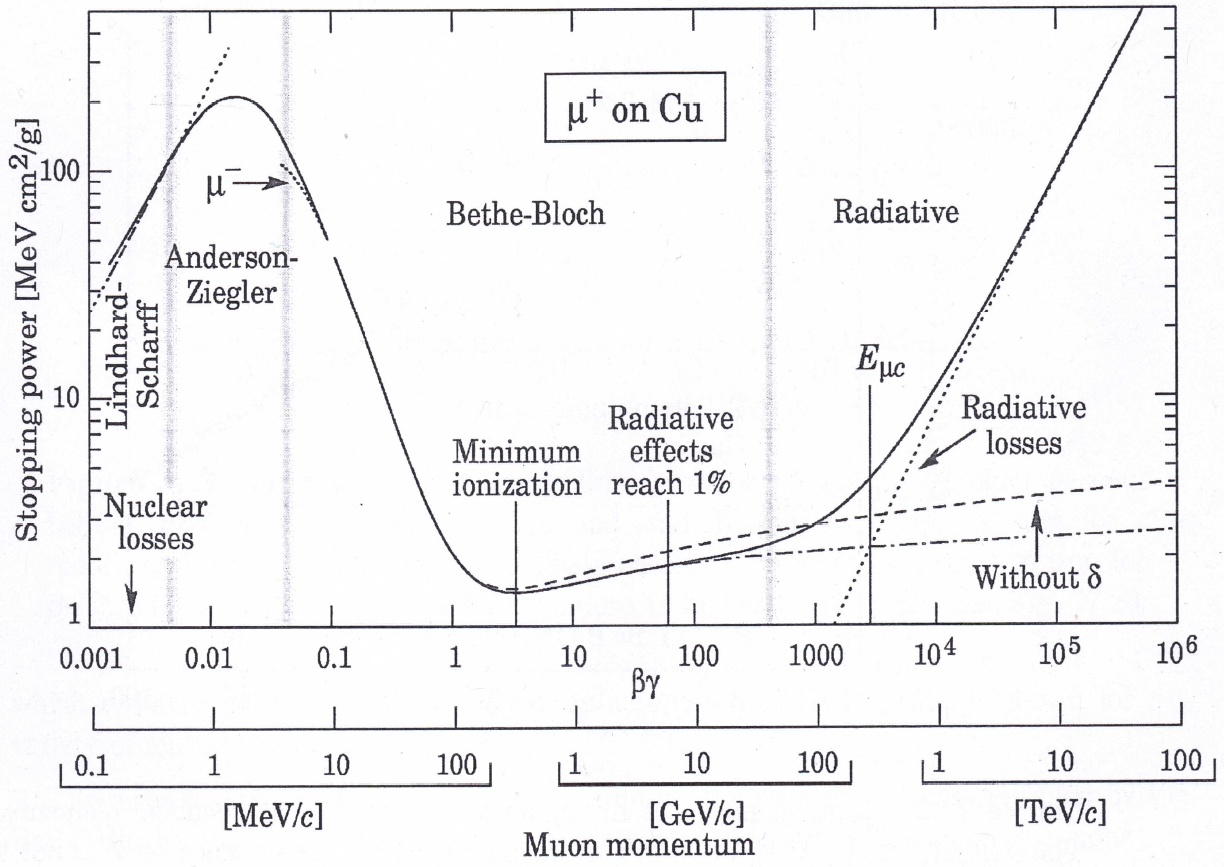
\includegraphics[width=\textwidth]{img/BetheBloch}
	\caption{Beispielhafter Kurvenverlauf der Bethe-Bloch-Formel für Myonen in Kupfer. Der Energieverlust ist auf Energie pro Strecke und Dichte normiert. \cite{bethebloch}}
	\label{bethebloch}
\end{figure}

Um die einzelnen Terme besser zu verstehen, wird eine sehr verkürzte Herleitung durch klassische Überlegungen vorgestellt.
Ein Teichen der Ladung $z\cdot e$, Masse $m$ und Geschwindigkeit $v$ fliege durch ein Medium und dabei an einem atomaren Elektron im Abstand $b$ vorbei.
Dieses Elektron sei ferner frei und anfangs in Ruhe.
Das eintreffende Teilchen werde außerdem aufgrund seiner viel größeren Masse ($M\gg m_e$) nicht aus seiner Bahn gelenkt.
Damit kann man nun den Impulsübertrag an das Elektron berechnen:
\begin{align*}
	I=\int F \dd{t}=e\int E_\perp \dd{t}=e\int E_\perp \dv{t}{x} \dd{x}=e\int E_\perp \frac{1}{v} \dd{x}=\frac{2ze^2}{bv}
\end{align*}
Das letzte Integral wurde mit dem Gauß'schen Integralsatz gelöst.
Die aufgenommene Energie des Elektrons ist damit gegeben durch:
\begin{align*}
	\Delta E(b)=\frac{I^2}{2m_e}=\frac{2z^2e^4}{m_e v^2b^2}
\end{align*}
Man führt nun die Elektronendichte $N_e$ ein.
Dann ist der infinitesimale Energieverlust eines Teilchens an Elektronen zwischen $b$ und $b+\text{d}b$ gegeben durch:
\begin{align*}
	-\text{d}E(b)=\Delta E(b)N_e \dd{V}= \frac{4\pi z^2e^4}{m_e v^2b}N_e \dd{b} \dd{x}
\end{align*}
Die Integration über $b$ lässt sich direkt ausführen:
\begin{align*}
	-\dv{E}{x}=\frac{4\pi z^2e^4}{m_e v^2}N_e\ln(\frac{b_\text{max}}{b_\text{min}})
\end{align*}
Die Werte von $b_\text{max}$ und $b_\text{min}$ lassen sich physikalisch begründen zu:
\begin{align*}
	b_\text{min}= \frac{ze^2}{\gamma m_e v^2}\qquad\text{und}\qquad b_\text{max}=\frac{\gamma v}{\bar{\nu}}
\end{align*}
Dabei ist $\bar{\nu}$ die mittlere Frequenz aller gebundenen Zustände.
Daraus ergibt sich die klassische Energieverlustformel nach Bohr.
Die Bethe-Bloch-Formel folgt mithilfe einiger quantenmechanischen Korrekturen, welche hier nicht im Detail besprochen werden sollen.

\begin{table}[h]
	\centering
	\caption{Auftauchende Größen in der Bethe-Bloch-Formel.}
	\begin{tabular}{cc}
		$r_e$: & klassischer Elektronenradius \\
		$m_e$: & Elektronenmasse \\
		$N_A$: & Avogadrokonstante \\
		$I$:  & mittleres Anregungspotential \\
		$Z$:  & Kernladungszahl Absorbermaterial \\
		$A$:  & Massenzahl Absorbermaterial \\
		$\rho$: & Dichte Absorbermaterial \\
		$z$:  & Ladungszahl des eintreffenden Teilchens \\
		$\beta$: & $v/c$ des eintreffenden Teilchens \\
		$\gamma$: & $1/\sqrt{1-\beta^2}$ \\
		$\delta$: & Dichte-Korrekturfaktor \\
		$C$:  & Schalen-Korrekturfaktor \\
		$W_\text{max}$: & max. Energietransfer pro einzelner Kollision \\
	\end{tabular}%
	\label{tab:bethebloch}%
\end{table}%

Für die Auswertung der Bethe-Bloch-Formel sind zusätzlich folgende Zusammenhänge notwendig:
\begin{align}
	W_\text{max}\approx 2m_ev^2\gamma^2\qquad\text{für }M\gg m_e
\end{align}
Der Dichte-Korrekturfaktor lautet:
\begin{align}
	\delta=\begin{cases}
	0 &\qquad\text{für }X<X_0\\
	4,6052\cdot X + C_0 + a(X_1-X)^m &\qquad\text{für }X_0<X<X_1\\
	4,6052\cdot X + C_0  &\qquad\text{für }X>X_1
	\end{cases}
\end{align}
Hierbei ist $X=\log_{10}(\beta \gamma)$.
Für Silizium sind $I=\SI{173}{\electronvolt}$, $C_0=\num{-4,44}$, $a=\num{0,1492}$, $m=\num{3,25}$, $X_1=\num{2,87}$ und $X_0=\num{0,2014}$ \cite{bethebloch}.
Der  Schalen-Korrekturfaktor lautet:
\begin{align}
	C(I,\eta=\beta\gamma)=(0,422377\,\eta^{-2}+0,0304043\,\eta^{-4}-0,00038106\,\eta^{-6})\cdot 10^{-6}\,I^2 \nonumber\\
	+(3,850190\,\eta^{-2}-0,1667989\,\eta^{-4}+0,00157955\,\eta^{-6})\cdot 10^{-9}\,I^3
\end{align}
Ferner gilt
\begin{align}
	\gamma = 1 + \frac{E_\text{kin}}{mc^2}\qquad\text{und}\qquad\beta=\sqrt{1-\frac{1}{\gamma^2}}.
\end{align}

\subsubsection{Bragg-Peak}

%Aus dieser Abhängigkeit des Energieverlustes folgt die sogenannte Bragg-Kurve.
%Diese stellt den Energieverlust pro zurückgelegtem Weg dar.
%Wie in Abbildung \ref{bragg} am Beispiel von Alpha-Teilchen in Luft zu sehen, ist der Energieverlust zunächst gering, da die Teilchen noch relativ viel Energie besitzen.
%Mit abnehmender Energie steigt der Energieverlust weiter an und die Teilchen verlieren die meiste Energie ganz zum Schluss am Bragg-Peak. % TODO sonst muss dieser Satz neu geschrieben werden

% das folgende erklärt den bragg peak durch die bethebloch formel % TODO checken!
Trifft ein geladenes Teilchen aus einem Kernprozess auf Materie, so wird dieser Prozess in der Bethe-Bloch-Formel zunächst durch den Bereich zwischen dem Anderson-Ziegler-Peak und der minimalen Ionisation beschrieben.
Die Energie des Teilchens nimmt ab und in Folge dessen erhöht sich der Energieverlust.
Da Abbildung \ref{bethebloch} eine logarithmische Darstellung ist, wächst der Energieverlust exponentiell mit der zurückgelegten Strecke an.
Hat das Teilchen beinahe seine gesamte Energie verloren, nimmt der Energieverlust schnell ab, was in Abbildung \ref{bethebloch} durch den Lindhard-Scharff-Bereich deutlich wird.
Die resultierende Bragg-Kurve ist so durch den langgezogenen niedrigen Energieverlust und den Bragg-Peak charakterisiert.
Die Kurvenform ist stark von Ladung, Masse und Energie des eintreffenden Teilchens, sowie der Dichte und Ladung des Absorbermaterials abhängig.
In Abbildung \ref{bragg} ist beispielhaft die Bragg-Kurve von $\alpha$-Teilchen in Luft gezeigt.

\begin{figure}[H]
	\centering
	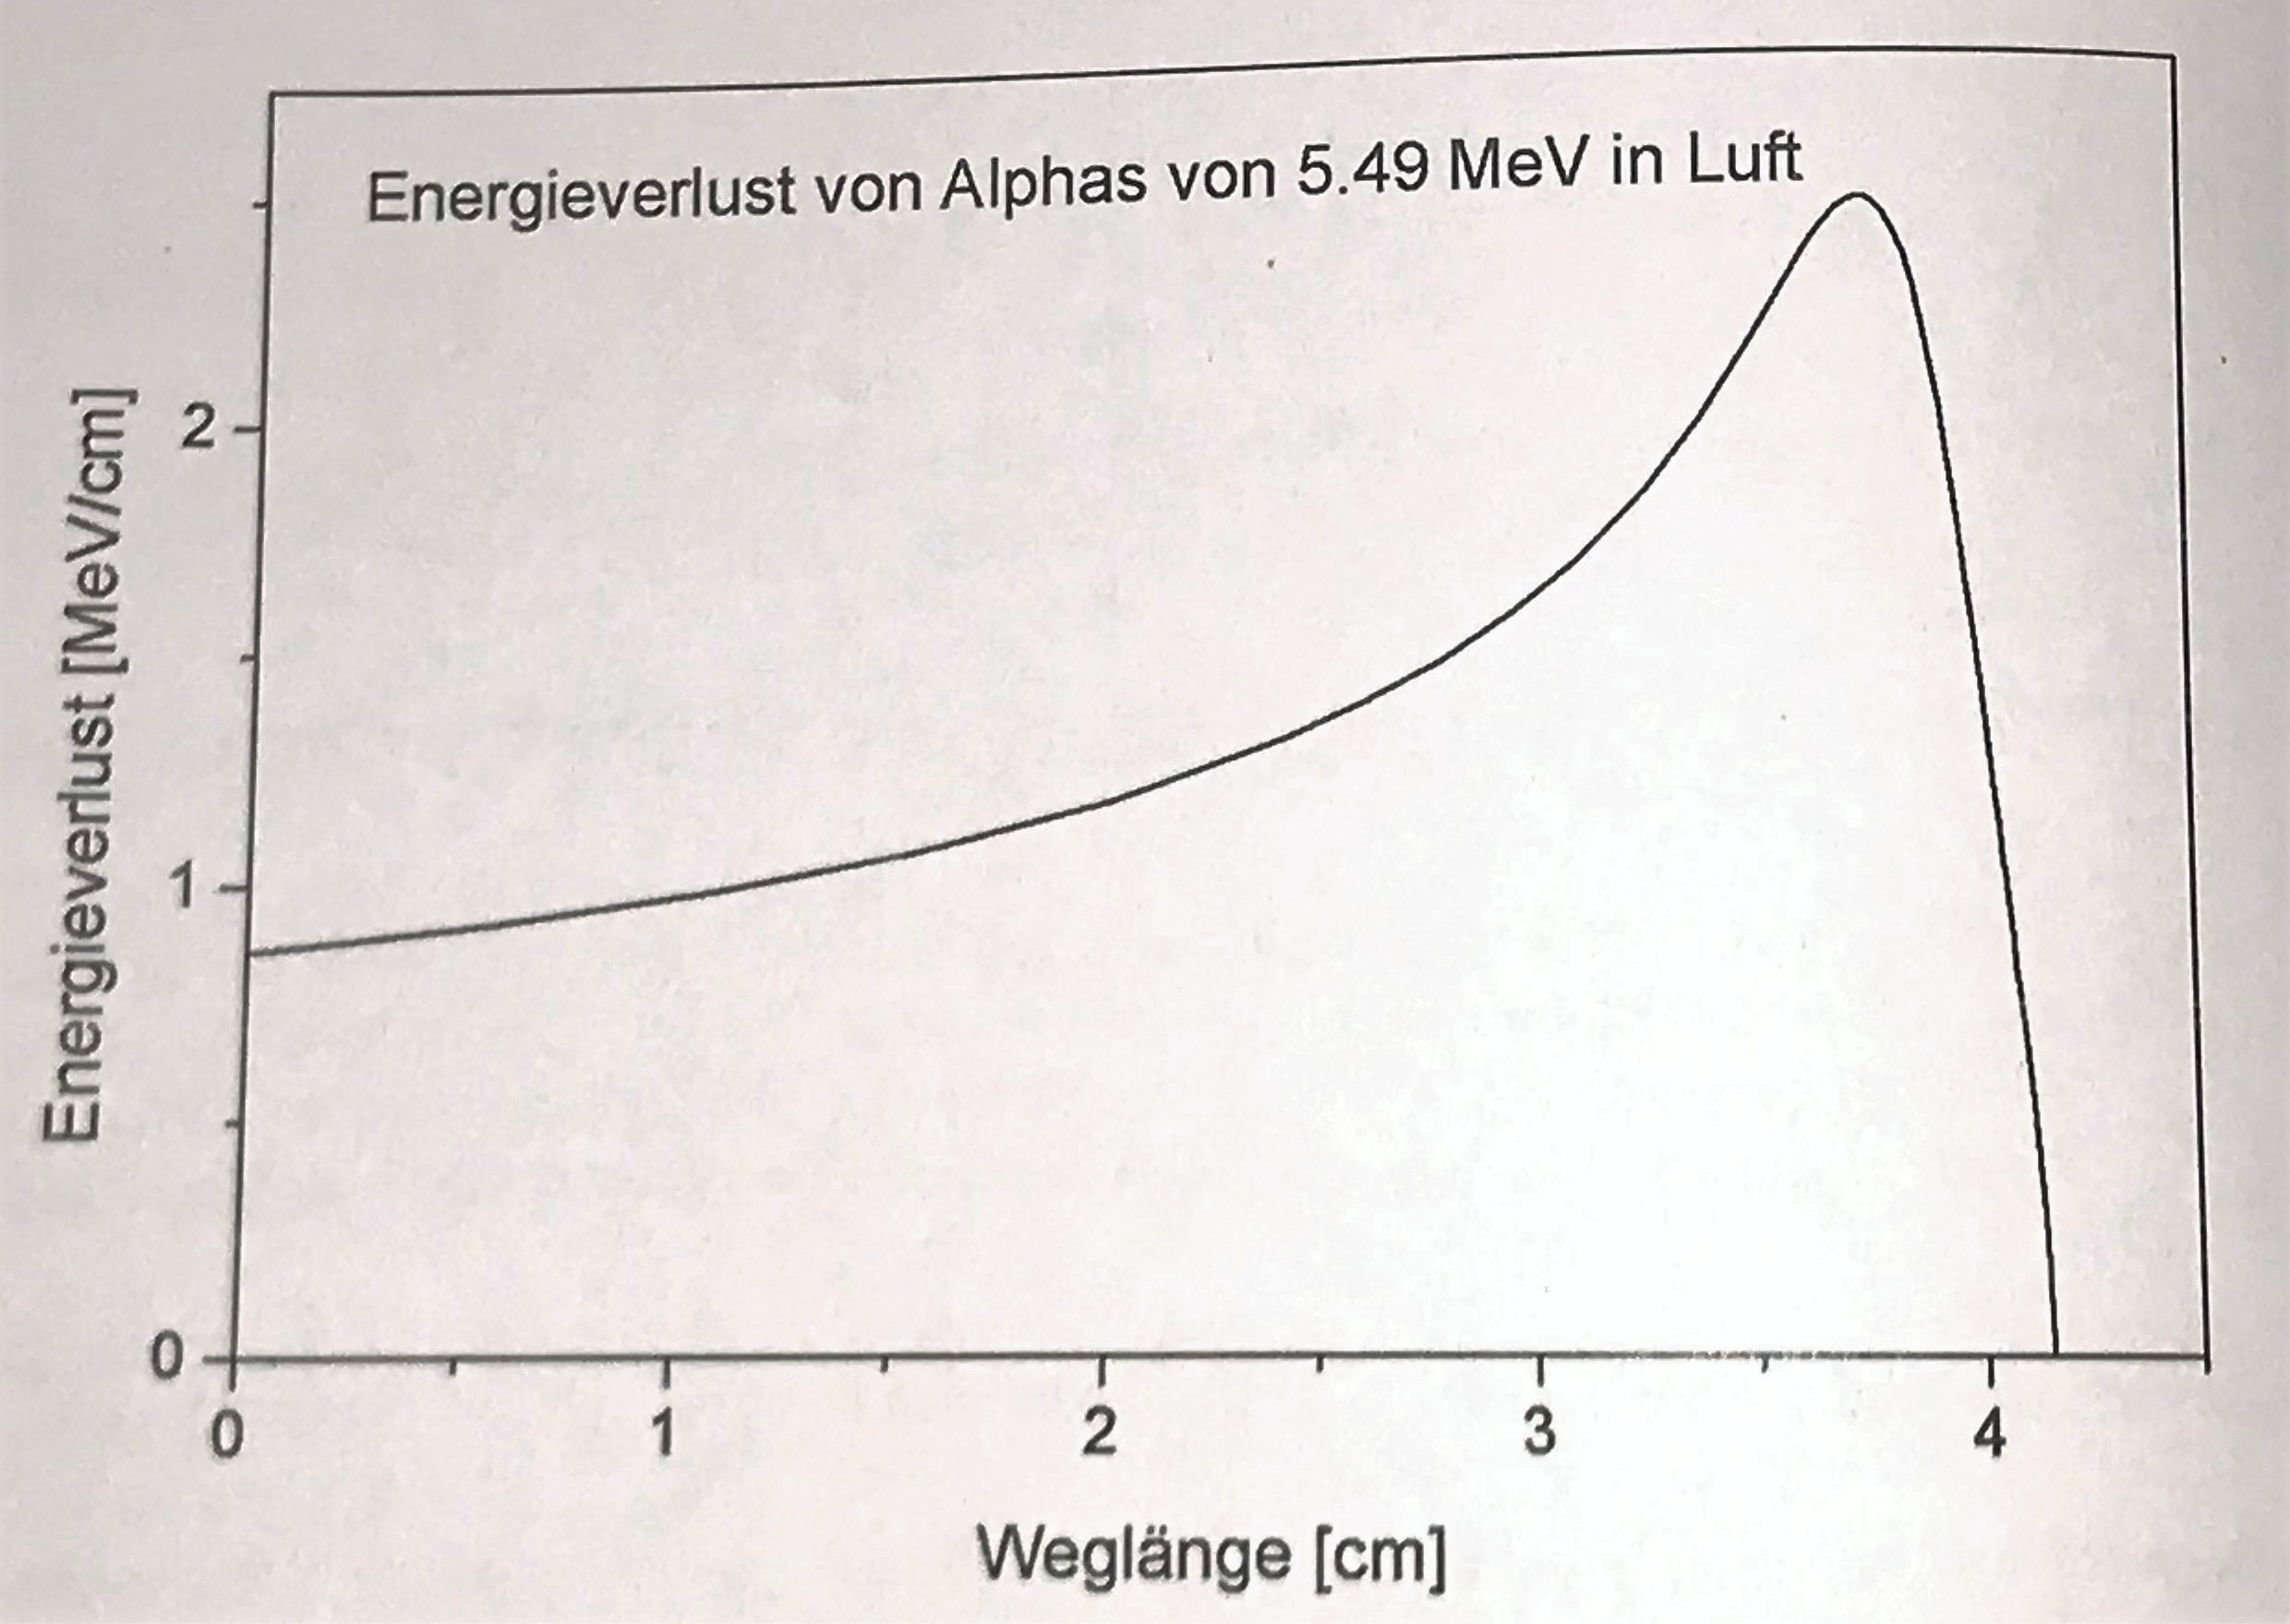
\includegraphics[width=0.8\textwidth]{img/bragg}
	\caption{Bragg-Peak von Alpha-Teilchen in Luft.\cite{bragg}}
	\label{bragg}
\end{figure}

\subsection{Halbleiter-Detektoren}

Ein Halbleiter-Detektor funktioniert ähnlich zu einer Gas-Ionisationskammer.
Im Gegensatz dazu werden jedoch nicht die Ionisationen eines Gases gemessen, sondern die erzeugten Elektron-Loch-Paare in der Sperrschicht einer Halbleiter-Diode.
Die zum Hervorrufen einer Reaktion notwendige Energie ist bei einem Halbleiter-Detektor um eine Größenordnung kleiner, was zu mehr freien Ladungen und einer kleineren statistischen Schwankung führt.
Zum besseren Verständnis von Halbleiter-Detektoren werden im Folgenden einige Grundlagen zu Halbleitern und pn-Übergängen vorgestellt.

\subsubsection{Halbleiter}

Im Gegensatz zu Leitern zeichnen sich Halbleiter dadurch aus, dass sie eine Bandlücke zwischen Valenz- und Leitungsband besitzen.
Diese Bandlücke ist bei Raumtemperatur ($T=\SI{300}{\kelvin}$) gerade klein genug ($\sim \si{\electronvolt}$, abhängig vom Halbleitermaterial und der Temperatur), um Elektronen durch thermische Anregung des Materials vom Valenz- ins Leitungsband zu heben.
Im Vergleich zu Halbleitern ist die Bandlücke bei Isolatoren wiederum um ein Vielfaches größer.
In den folgenden Experimenten wird mit Silizium ein elementarer Halbleiter der vierten Hauptgruppe des Periodensystems betrachtet.
Andere Halbleiter wie Galliumarsenid sind beispielsweise aus Elementen der dritten und fünften Hauptgruppe zusammengesetzt.

Bei Raumtemperatur ist der spezifische Widerstand eines Halbleiters groß, da sich nach dem Bändermodell nur wenige Ladungsträger im Leitungsband befinden.
Durch das Einbringen von Elementen der fünften Hauptgruppe (Donatoren) in das (Halbleiter-) Kristallgitter kommt eine sogenannte n-Dotierung zustande.
Dabei besitzt das eingebrachte Element ein negativ geladenes Elektron zu viel in der äußeren Schale, um sich optimal in das Kristallgitter einfügen zu können.
Dies führt dazu, dass dieses Elektron nicht fest an den Atomrumpf gebunden ist und durch thermische Anregung leicht ins Leitungsband befördert werden kann.
Somit sinkt der spezifische Widerstand und die Leitfähigkeit steigt.
Ebenso kann mit Elementen der dritten Hauptgruppe (Akzeptoren) eine sogenannte p-Dotierung erreicht werden.
Dadurch kommt es zu fehlenden Elektronen im (Halbleiter-) Kristallgitter, sodass mit einer geringen thermischen Anregung ein Elektron von einem benachbarten Atom an diese Fehlstelle springen kann.
Nun liegt die Fehlstelle aber am Nachbar-Atom vor, zu der wiederum ein Elektron eines anderen Atoms springen kann.
Es handelt sich also um ein "bewegliches Loch", was einem Ladungstransport ("Löcherbewegung") gleichkommt.
Daher sinkt der spezifische Widerstand und die Leitfähigkeit steigt.


\subsubsection{Der pn-Übergang}

Für den Übergang zum Halbleiter-Detektor ist der sogenannte pn-Übergang entscheidend.
Bei Verwendung als elektrisches Bauteil wird er dabei auch als Diode bezeichnet.
Kommen ein p- und ein n-dotierter Halbleiter in Kontakt sorgen die unterschiedlichen Konzentrationen von Elektronen und Löchern dafür, dass die Majoritätsladungsträger in die jeweils anders dotierte Halbleiterschicht diffundieren und dort rekombinieren.
Die Atomrümpfe bleiben hingegen an ihren Positionen, wodurch sich im n-dotierten Bereich eine positive Raumladung und im p-dotierten Bereich eine negative Raumladung ergibt.
Dieses Potentialgefälle erzeugt im Inneren der Diode eine sogenannte Raumladungszone, welche einer weiteren Diffusion von Majoritätsladungstägern offensichtlich entgegen wirkt.

Im thermodynamischen Gleichgewicht halten sich diese beiden Prozesse die Waage.
Das heißt, die Summe des Diffusionsstroms und des entgegengesetzten, durch die Raumladungszone erzeugten Driftstroms ist gleich null.
Dies führt auf eine lineare Differentialgleichung erster Ordnung, deren Lösung die bekannte Kennlinie einer Diode ist:
\begin{align}
I=I_0\cdot\left[ \exp\left( \frac{e\,U}{n\,k_\text{B}\,T}\right)  -1\right] 
\end{align} 

\noindent Dabei ist $k_\text{B}$  die Boltzmannkonstante,
$T$ die Temperatur in K, 
$I_0$ der Sättigungsstrom, abhängig von Materialparametern und der Temperatur, sowie
$n$ der Idealitätsfaktor mit $ 1 \leq n < 2$.
Er beschreibt die Ausdehnung der Raumladungszone.
Bei kleiner Ausdehnung ist $n = 1$ eine gute Näherung.

Liegt der n-Bereich auf positivem Potential $(U<0)$ wird die Diffusionsspannung $-U_\textnormal{Diff}$ verstärkt: Man gerät in den Sperrbereich.
Bei sehr hoher Sperrspannungen wird der Stromfluss wird alleine durch den Driftstrom der Minoritätsladungen bestimmt $(I\approx I_0)$.
Bei Polung der Diode in Flussrichtung $(U > 0)$ wird die Diffusionsspannung abgebaut und der Stromfluss wächst exponentiell.
Bei einer realen Diode müssen außerdem noch Korrekturen durch auftretende Leistungsverluste vorgenommen werden.
Diese werden beschrieben durch einen Parallel-/Shuntwiderstand $R_{\textnormal{sh}}$ und einen Serienwiderstand $R_{\textnormal{s}}$:
\begin{align}
I=I_0\cdot\left[ \exp\left( \frac{e\,(U-I\,R_\textnormal{s})}{n\,k_\textnormal{B}\,T}\right)  -1\right] +\frac{(U-I\,R_\textnormal{s})}{R_\textnormal{sh}}
\end{align} 


\subsection{Americium-241 als Quelle}

Die im Experiment verwendete Quelle ist $^{241}$Am.
Aufgrund der Lebensdauer
von 432,2 Jahren kann es nicht mehr aus der Natur gewonnen werden, sondern muss synthetisiert werden.
Durch Emission eines $\alpha$-Teilchens zerfällt es in $^{237}$Np (Neptunium).
Außerdem besteht die Möglichkeit einer spontanen Kernspaltung, jedoch ist die Wahrscheinlichkeit so gering, dass sie hier vernachlässigt werden kann.

Nach dem Zerfall liegt das entstehende $^{237}$Np nur selten im Grundzustand vor.
Mit einer Wahrscheinlichkeit von ca. \SI{84,45(10)}{\percent} zerfällt das Americium in den zweiten angeregten Zustand von Neptunium.
Die aus der Energie- und Impulserhaltung bei einem Zweikörperzerfall resultierende Energie für die Alpha-Teilchen ist damit:
\begin{align*}
	E_\alpha = \SI{5485,56(12)}{\kilo\electronvolt}.
\end{align*}